\documentclass[tikz,border=9pt]{standalone}
\usepackage{fontspec}
\setsansfont{Humor Sans}
\renewcommand{\familydefault}{\sfdefault}
\usepackage{tikz}
\usetikzlibrary{decorations.pathmorphing}

\definecolor{colBlue}{HTML}{2F6FB5}
\definecolor{colRed}{HTML}{C93A31}
\definecolor{colOrange}{HTML}{C87A0A}
\definecolor{colGreen}{HTML}{227A32}
\definecolor{colPurple}{HTML}{7A4FA3}
\definecolor{colTeal}{HTML}{127F87}
\definecolor{colAccent}{HTML}{3B3A8F}
\definecolor{colGray}{HTML}{5A5A5A}

\def\subfont{\fontsize{11pt}{13pt}\selectfont}
\def\capfont{\fontsize{7pt}{8.8pt}\selectfont}
\def\hdffont{\fontsize{8pt}{10pt}\selectfont}
\def\grpfont{\fontsize{8pt}{10pt}\selectfont}
\def\rowfont{\fontsize{8.5pt}{10.5pt}\selectfont}

\pgfmathsetseed{7}

% wiggly rule: [style] x0 / x1 / y
\newcommand{\wrule}[4][line width=0.9pt]{%
  \draw[#1, decorate, decoration={random steps, segment length=7pt, amplitude=0.55pt}]
    (#2,#4) -- (#3,#4);}

% TFLOPS bars, left table scaled to 250, right tables to 250 / 210
\newcommand{\lbar}[3]{%
  \pgfmathsetmacro{\bw}{#2/250*1.8}%
  \fill[#3] (5.95,{#1-0.075}) rectangle ++(\bw cm,0.15);}
\newcommand{\rbarA}[3]{%
  \pgfmathsetmacro{\bw}{#2/250*1.65}%
  \fill[#3] (14.80,{#1-0.075}) rectangle ++(\bw cm,0.15);}
\newcommand{\rbarB}[3]{%
  \pgfmathsetmacro{\bw}{#2/210*1.65}%
  \fill[#3] (14.80,{#1-0.075}) rectangle ++(\bw cm,0.15);}

% data row: y / config / TFLOPS / speedup / color
\newcommand{\lrow}[5]{%
  \node[anchor=west, font=\rowfont, inner sep=0pt] at (0,#1) {#2};%
  \node[anchor=east, font=\rowfont, inner sep=0pt] at (4.20,#1) {#3};%
  \node[anchor=east, font=\rowfont, inner sep=0pt, text=#5] at (5.60,#1) {#4};%
  \lbar{#1}{#3}{#5}}

\newcommand{\rrowA}[5]{%
  \node[anchor=west, font=\rowfont, inner sep=0pt] at (8.60,#1) {#2};%
  \node[anchor=east, font=\rowfont, inner sep=0pt] at (13.10,#1) {#3};%
  \node[anchor=east, font=\rowfont, inner sep=0pt, text=#5] at (14.50,#1) {#4};%
  \rbarA{#1}{#3}{#5}}

\newcommand{\rrowB}[5]{%
  \node[anchor=west, font=\rowfont, inner sep=0pt] at (8.60,#1) {#2};%
  \node[anchor=east, font=\rowfont, inner sep=0pt] at (13.10,#1) {#3};%
  \node[anchor=east, font=\rowfont, inner sep=0pt, text=#5] at (14.50,#1) {#4};%
  \rbarB{#1}{#3}{#5}}

% group heading: separated? / y / color / text
\newcommand{\lgrp}[4]{%
  \ifnum#1=1 \wrule[draw=black!20, line width=0.5pt]{0}{7.75}{#2+0.30}\fi
  \fill[#3] (0,{#2-0.075}) rectangle ++(0.17,0.17);%
  \node[anchor=west, font=\grpfont, inner sep=0pt, text=#3] at (0.30,#2) {#4};}
\newcommand{\rgrp}[4]{%
  \ifnum#1=1 \wrule[draw=black!20, line width=0.5pt]{8.60}{17.55}{#2+0.30}\fi
  \fill[#3] (8.60,{#2-0.075}) rectangle ++(0.17,0.17);%
  \node[anchor=west, font=\grpfont, inner sep=0pt, text=#3] at (8.90,#2) {#4};}

\begin{document}
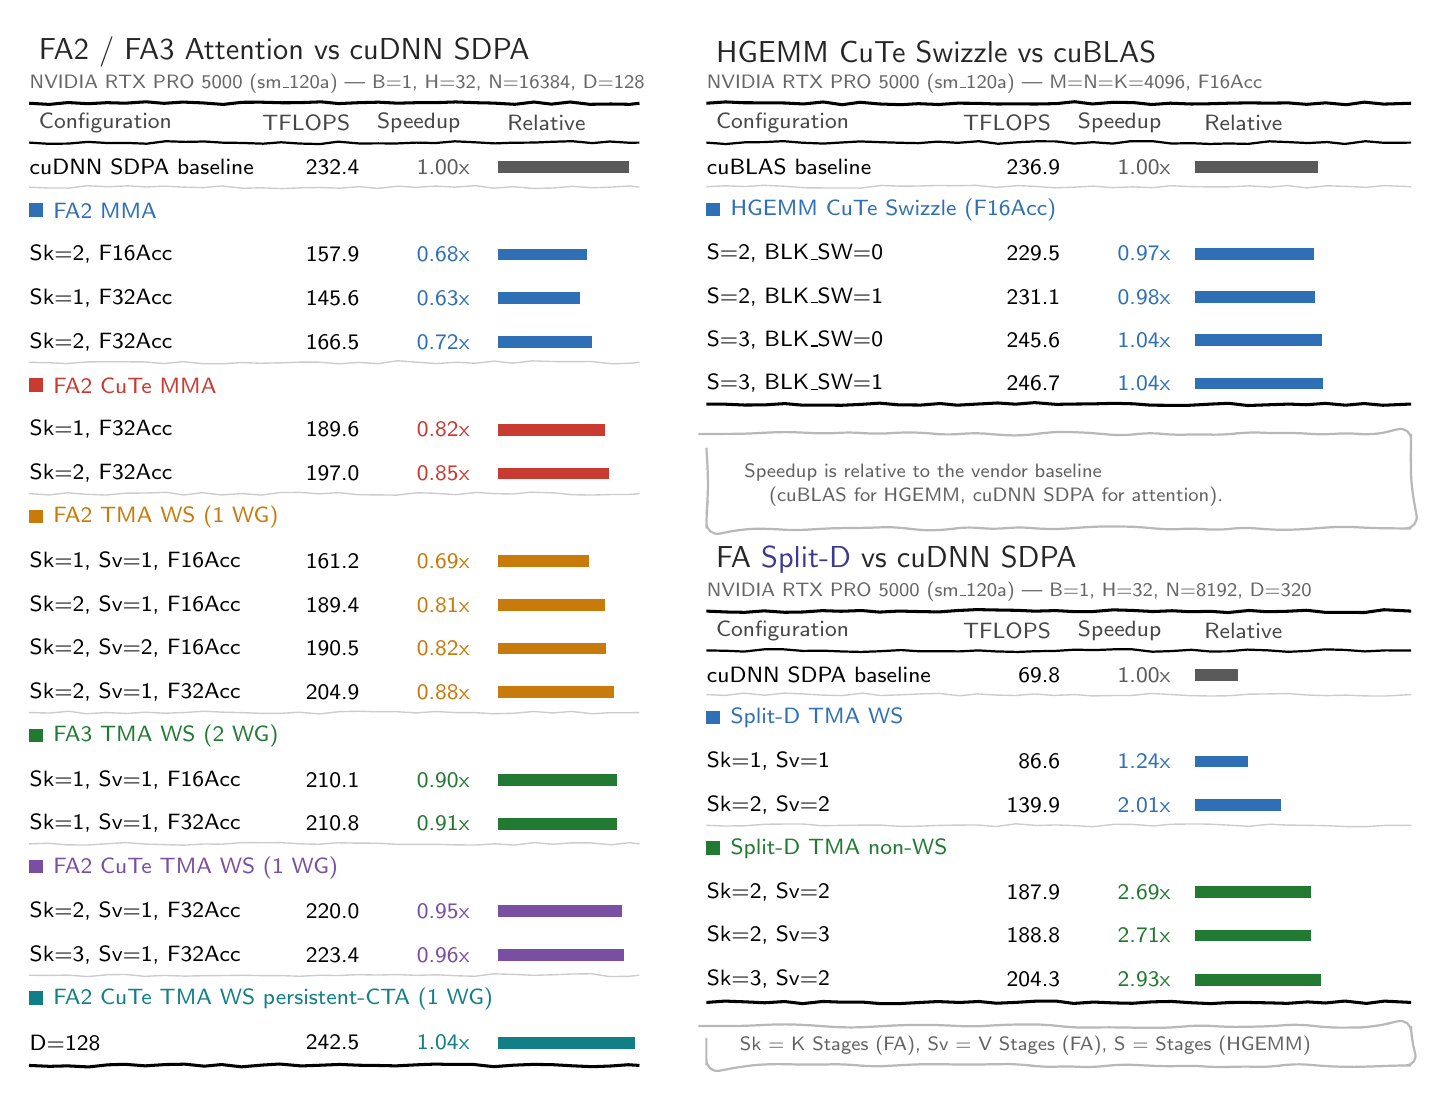
\begin{tikzpicture}

% ===================== LEFT: FA2 / FA3 vs cuDNN SDPA =====================
\node[anchor=west, font=\subfont, text=black!85] at (0,-0.35)
  {FA2 / FA3 Attention vs cuDNN SDPA};
\node[anchor=north west, font=\capfont, text=black!60, align=left, inner sep=0pt] at (0,-0.62)
  {NVIDIA RTX PRO 5000 (sm\_120a) --- B=1, H=32, N=16384, D=128};

\wrule[line width=1.1pt]{0}{7.75}{-1.00}
\node[anchor=west, font=\hdffont, text=black!72] at (0,-1.25) {Configuration};
\node[anchor=east, font=\hdffont, text=black!72] at (4.20,-1.25) {TFLOPS};
\node[anchor=east, font=\hdffont, text=black!72] at (5.60,-1.25) {Speedup};
\node[anchor=west, font=\hdffont, text=black!72] at (5.95,-1.25) {Relative};
\wrule[line width=0.8pt]{0}{7.75}{-1.50}

\lrow{-1.810}{cuDNN SDPA baseline}{232.4}{1.00x}{colGray}

\lgrp{1}{-2.366}{colBlue}{FA2 MMA}
\lrow{-2.922}{Sk=2, F16Acc}{157.9}{0.68x}{colBlue}
\lrow{-3.478}{Sk=1, F32Acc}{145.6}{0.63x}{colBlue}
\lrow{-4.034}{Sk=2, F32Acc}{166.5}{0.72x}{colBlue}

\lgrp{1}{-4.590}{colRed}{FA2 CuTe MMA}
\lrow{-5.146}{Sk=1, F32Acc}{189.6}{0.82x}{colRed}
\lrow{-5.702}{Sk=2, F32Acc}{197.0}{0.85x}{colRed}

\lgrp{1}{-6.258}{colOrange}{FA2 TMA WS (1 WG)}
\lrow{-6.814}{Sk=1, Sv=1, F16Acc}{161.2}{0.69x}{colOrange}
\lrow{-7.370}{Sk=2, Sv=1, F16Acc}{189.4}{0.81x}{colOrange}
\lrow{-7.926}{Sk=2, Sv=2, F16Acc}{190.5}{0.82x}{colOrange}
\lrow{-8.482}{Sk=2, Sv=1, F32Acc}{204.9}{0.88x}{colOrange}

\lgrp{1}{-9.038}{colGreen}{FA3 TMA WS (2 WG)}
\lrow{-9.594}{Sk=1, Sv=1, F16Acc}{210.1}{0.90x}{colGreen}
\lrow{-10.150}{Sk=1, Sv=1, F32Acc}{210.8}{0.91x}{colGreen}

\lgrp{1}{-10.706}{colPurple}{FA2 CuTe TMA WS (1 WG)}
\lrow{-11.262}{Sk=2, Sv=1, F32Acc}{220.0}{0.95x}{colPurple}
\lrow{-11.818}{Sk=3, Sv=1, F32Acc}{223.4}{0.96x}{colPurple}

\lgrp{1}{-12.374}{colTeal}{FA2 CuTe TMA WS persistent-CTA (1 WG)}
\lrow{-12.930}{D=128}{242.5}{1.04x}{colTeal}

\wrule[line width=1.1pt]{0}{7.75}{-13.22}

% ===================== RIGHT TOP: HGEMM vs cuBLAS =====================
\node[anchor=west, font=\subfont, text=black!85] at (8.60,-0.35)
  {HGEMM CuTe Swizzle vs cuBLAS};
\node[anchor=north west, font=\capfont, text=black!60, align=left, inner sep=0pt] at (8.60,-0.62)
  {NVIDIA RTX PRO 5000 (sm\_120a) --- M=N=K=4096, F16Acc};

\wrule[line width=1.1pt]{8.60}{17.55}{-1.00}
\node[anchor=west, font=\hdffont, text=black!72] at (8.60,-1.25) {Configuration};
\node[anchor=east, font=\hdffont, text=black!72] at (13.10,-1.25) {TFLOPS};
\node[anchor=east, font=\hdffont, text=black!72] at (14.50,-1.25) {Speedup};
\node[anchor=west, font=\hdffont, text=black!72] at (14.80,-1.25) {Relative};
\wrule[line width=0.8pt]{8.60}{17.55}{-1.50}

\rrowA{-1.810}{cuBLAS baseline}{236.9}{1.00x}{colGray}

\rgrp{1}{-2.360}{colBlue}{HGEMM CuTe Swizzle (F16Acc)}
\rrowA{-2.910}{S=2, BLK\_SW=0}{229.5}{0.97x}{colBlue}
\rrowA{-3.460}{S=2, BLK\_SW=1}{231.1}{0.98x}{colBlue}
\rrowA{-4.010}{S=3, BLK\_SW=0}{245.6}{1.04x}{colBlue}
\rrowA{-4.560}{S=3, BLK\_SW=1}{246.7}{1.04x}{colBlue}

\wrule[line width=1.1pt]{8.60}{17.55}{-4.82}

\node[anchor=north west, font=\capfont, text=black!62, align=left, inner sep=5pt]
  at (8.90,-5.40) {Speedup is relative to the vendor baseline\\\hspace*{1.2em}(cuBLAS for HGEMM, cuDNN SDPA for attention).};
\draw[draw=black!28, line width=0.8pt, decorate,
      decoration={random steps, segment length=9pt, amplitude=0.8pt}, rounded corners=5pt]
  (8.60,-5.20) rectangle (17.55,-6.40);

% ===================== RIGHT BOTTOM: FA Split-D vs cuDNN SDPA =====================
\node[anchor=west, font=\subfont, text=black!85] at (8.60,-6.80)
  {FA \textcolor{colAccent}{Split-D} vs cuDNN SDPA};
\node[anchor=north west, font=\capfont, text=black!60, align=left, inner sep=0pt] at (8.60,-7.07)
  {NVIDIA RTX PRO 5000 (sm\_120a) --- B=1, H=32, N=8192, D=320};

\wrule[line width=1.1pt]{8.60}{17.55}{-7.45}
\node[anchor=west, font=\hdffont, text=black!72] at (8.60,-7.70) {Configuration};
\node[anchor=east, font=\hdffont, text=black!72] at (13.10,-7.70) {TFLOPS};
\node[anchor=east, font=\hdffont, text=black!72] at (14.50,-7.70) {Speedup};
\node[anchor=west, font=\hdffont, text=black!72] at (14.80,-7.70) {Relative};
\wrule[line width=0.8pt]{8.60}{17.55}{-7.95}

\rrowB{-8.26}{cuDNN SDPA baseline}{69.8}{1.00x}{colGray}

\rgrp{1}{-8.81}{colBlue}{Split-D TMA WS}
\rrowB{-9.36}{Sk=1, Sv=1}{86.6}{1.24x}{colBlue}
\rrowB{-9.91}{Sk=2, Sv=2}{139.9}{2.01x}{colBlue}

\rgrp{1}{-10.47}{colGreen}{Split-D TMA non-WS}
\rrowB{-11.02}{Sk=2, Sv=2}{187.9}{2.69x}{colGreen}
\rrowB{-11.57}{Sk=2, Sv=3}{188.8}{2.71x}{colGreen}
\rrowB{-12.13}{Sk=3, Sv=2}{204.3}{2.93x}{colGreen}

\wrule[line width=1.1pt]{8.60}{17.55}{-12.42}

\node[anchor=west, font=\capfont, text=black!62, inner sep=0pt] at (9.02,-12.97)
  {Sk = K Stages (FA), Sv = V Stages (FA), S = Stages (HGEMM)};
\draw[draw=black!28, line width=0.8pt, decorate,
      decoration={random steps, segment length=9pt, amplitude=0.8pt}, rounded corners=5pt]
  (8.60,-12.72) rectangle (17.55,-13.22);

\end{tikzpicture}
\end{document}
